\documentclass[12pt, landscape]{article}
\usepackage[scaled=0.92]{helvet}
\usepackage{multicol}
\usepackage{calc}
\usepackage{ifthen}
\usepackage[landscape]{geometry}
%\usepackage{hyperref}

\usepackage{newtxtext} 

%for strikeout
\usepackage{ulem}

%For editing parbox
\usepackage[table]{xcolor}
%For editing itemise margins, reduce iterm separaion and list separation
\usepackage{enumitem}
% For math
\usepackage{amsmath,amsthm,amsfonts,amssymb}

%For pictures / figures
\usepackage{color,graphicx,overpic}
\graphicspath{ {./images/} }

%\usepackage{newtxtext} 
%\usepackage{amssymb}
%\usepackage[table]{xcolor}
%\usepackage{vwcol}
%\usepackage{tikz}
%\usepackage{wrapfig}
%\usepackage{makecell}

\pdfinfo{
  /Title (IS2238.pdf)
  /Creator (Ger Teck)
  /Author (Ger Teck)
  /Subject ()
  /Keywords (tex)}

%% Margins for PAPER

% This sets page margins to .5 inch if using letter paper, and to 1cm
% if using A4 paper. (This probably isn't strictly necessary.)
% If using another size paper, use default 1cm margins.
\ifthenelse{\lengthtest { \paperwidth = 11in}}
	{ \geometry{top=.5in,left=.5in,right=.5in,bottom=.5in} }
	{\ifthenelse{ \lengthtest{ \paperwidth = 297mm}}
		{\geometry{top=1cm,left=1cm,right=1cm,bottom=1cm} }
		{\geometry{top=1cm,left=1cm,right=1cm,bottom=1cm} }
	}

% Turn off header and footer
\pagestyle{empty}

% for tight centres (less spacing)
\newenvironment{tightcenter}{%
  \setlength\topsep{0pt}
  \setlength\parskip{0pt}
  \begin{center}
}{%
  \end{center}
}

% Redefine section commands to use less space
\makeatletter
\renewcommand{\section}{\@startsection{section}{1}{0mm}%
                                {-1ex plus -.5ex minus -.2ex}%
                                {0.5ex plus .2ex}%x
                                {\normalfont\large\bfseries}}
\renewcommand{\subsection}{\@startsection{subsection}{2}{0mm}%
                                {-1explus -.5ex minus -.2ex}%
                                {0.5ex plus .2ex}%
                                {\normalfont\normalsize\bfseries}}
\renewcommand{\subsubsection}{\@startsection{subsubsection}{3}{0mm}%
                                {-1ex plus -.5ex minus -.2ex}%
                                {1ex plus .2ex}%
                                {\normalfont\small\bfseries}}
% change font
%\renewcommand{\familydefault}{\sfdefault}
%\renewcommand\rmdefault{\sfdefault}
\makeatother

% Define BibTeX command
\def\BibTeX{{\rm B\kern-.05em{\sc i\kern-.025em b}\kern-.08em
    T\kern-.1667em\lower.7ex\hbox{E}\kern-.125emX}}

% Don't print section numbers
\setcounter{secnumdepth}{0}

\setlength{\parindent}{0pt}
\setlength{\parskip}{0pt plus 0.5ex}

%% this changes all items (enumerate and itemize, reduce margins)
\setlength{\leftmargini}{0.5cm}
\setlength{\leftmarginii}{0.5cm}
\setlist[itemize,1]{leftmargin=2mm,labelindent=1mm,labelsep=1mm, itemsep = 2mm}
\setlist[itemize,2]{leftmargin=4mm,labelindent=1mm,labelsep=1mm, itemsep = 2mm}
\itemsep = 3mm
%\setlist{nosep}

% -------------------------------------------------------------------------------

% START OF DOCUMENT HERE

\begin{document}
\raggedright
\footnotesize
\begin{multicols*}{3}

% multicol parameters
% These lengths are set only within the two main columns
\setlength{\columnseprule}{0pt}
\setlength{\premulticols}{1pt}
\setlength{\postmulticols}{1pt}
\setlength{\multicolsep}{2pt}
\setlength{\columnsep}{2pt}

%% DOCUMENT NAME HERE
\begin{center}
     \Large{\textbf{IS2238 Economics of IT \& AI}} \\
\end{center}

% TABLE PACKAGE 
 \begin{center}
    \fbox{%
        \parbox{0.8\linewidth}{\centering \textcolor{black}{
            \\ \normalsize{AY22/23 Sem 2}}
            \\ {\footnotesize github.com/gerteck}
        }%
    }
  \end{center}

\section{1. Overview of Economics of IT}

\begin{itemize}
	\item \textbf{IT/AI are changing our lives, businesses, and economy.} Economics can provide a lens through which we can better understand this new economy and phenomena in a more systematic manner.
	\item High speed change in today’s digital age. (Digital revolution). Cause of change is computer \& comunications, technology such as integreted circuits, data speed and laptop capacity which have increased by many times. $\rightarrow$ Increase in employee productivity.
	\item \textbf{Moore’s Law:} observation that the numer of transistors on a microchip doubles every 18-24 months (exponential growth). Advancement has slowed down since 2010s.
	\item \textbf{Why does IT matter for today's economy?}: IT capital investment by companies has grown steadily over the years from 1980s to 2010. Market capitalization has seen most large companies being tech related or heavily invested in IT.
	\item \textbf{Economics:} Allows for systematic understanding of new phenomena. This provides a lens through which we can better understand how things work, design clever solutions and create the conditions in which we can all flourish. We do this through economic theory, methods, analytical methods, empricial modelling.
	\item \textbf{Evaluating IT investment and its impact:} IT investments by firms do not necessarily lead to better outcomes nor better lives. Question has important policy and managerial implications. There are many variables to consider, such as obsolescence of old technologies, cost of learning, infrastructures, poor IT management, underutilization. Companies need to throughly understand the role and impact of IT on their business models and the exact use if implemented.
	\item \textbf{IT Productivity Paradox}: Economist Robert Solow: a Nobel Prize laureate, famously said in 1987, “You can see the computer age everywhere but in the productivity statistics”. It was largely resolved by an economics analysis done by MIT professor Erik Brynjolfsson and his colleagues in in the mid-1990s. Cobb–Douglas production function.
\end{itemize}

\subsection{Cobb-Douglas Production Function} 
models the relationship between production output and production inputs (factors).
\centerline{$Y = AL^\beta K^\alpha$}
\\ Y: Total Production, L: Labor Input,
\\ K: Capital Input, A: Total Factor Productivity,
\\ $\alpha$ and $\beta$: output elasticities of capital and labour.
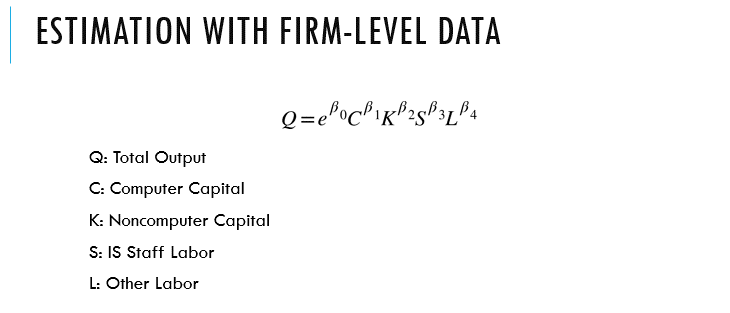
\includegraphics[width=\linewidth]{firmLevelData}

~\\

\textbf{Insights:} Brynjolfsson and Hitt (Management Science, 1996)
\begin{itemize}
\item An additional dollar of computer capital stock is associated with an increase in output of 81 cents per year on the margin An additional dollar spent was associated with a marginal increase in output of \$2.62
\end{itemize}


\section{2. Digital Economy and New IT}
\subsection{McKinsey View on 'New' IT}
\begin{itemize}
\item Numerous industries being `reimagined' through IT: To prevent a competitor from re-imagining your product as discontinued or re-imagining your company into liquidation, IT could well be an essential consideration in strategy formulation and execution, and a key area for investment.
\item `Old IT': Addressed labor automation, individual worker productivity, and non-human scale computing;
\item `New IT': Focus on digital products and services, team productivity, and business model transformation.
\item Benefits from old IT have reached a point of diminishing returns; new IT can be a source of competitive differentiation and dramatic wealth creation.
\item \textbf{Business Model Transformation} as a major use of IT, five major levers: Production and operations optimization, Eliminating intermediaries (bypassing middleman), New Monetization models (Amazon Web Services, SaaS etc.), Shaping customer preferences (leveraging big data), Transforming underserved markets (Long Tail phenomenon).
\end{itemize}

\subsection{Old Supply Chain Issues}
\begin{itemize}
\item Lack of Coordination between stages in the supply chain where objectives of different stages conflict or information moving between stages is distorted.
\item \textbf{Bullwhip Effect:} Fluctuations in order increases as they move up the supply chain from retailers to wholesalers to manufacturers to suppliers. Distorted demand information, where different stages have different estimates of what demand looks like, amplified variation in demand. Higher safety inventory usually required.
\item Information Processing Obstacles: Forecasting demand based on orders, not customer demand. Lack of information sharing. To overcome tradeoff, we trade responsiveness for cost and vice versa.
\end{itemize}

\subsection{Just-In-Time Production Methods}
\begin{itemize}
\item Tesla Motors has been using Just-In-Time (JIT) production methods to keep costs low since its founding in 2003. (JIT Benefits + Challenges) Tesla is experimenting with lean manufacturing principles in its production processes.
\item JIT is a production strategy that seeks to minimize waste and maximize efficiency by only producing what is needed, when it is needed. This approach requires close coordination between all parts of the production process, from suppliers to assembly line workers.
\item There are some challenges associated with JIT, such as the need for tight coordination and the potential for disruptions to the production process. However, Tesla has shown that JIT can be an effective production strategy for a high-tech manufacturing company.
\end{itemize}

\subsection{Digital Economy}
\begin{itemize}
\item \textbf{A Digital Economy} takes advantage of the latest technology to digitalise processes and drive business growth. With digital economy, most of economic activities such as production, distribution, and consumption of goods and services are digitalized.
\item Digital technologies reduce the cost of storage, computation, and transmission of data. Therefore, digital economics explores how standard economic models change as certain costs fall substantially and perhaps approach zero.
\item \textbf{IT Capital Investment:} IT Capital Investment by companies has been increasing (in proportion and amount) over the years. IT automate many steps in business processes that were formerly performed manually. IT can enable new innovative business processes by collecting, processing, distributing information in a more efficient and effective way. (e.g., JIT, cross-docking) IT can transform the way the business works and drive new business models.
\end{itemize}

\textbf{Production and Economics of Production: Cost Curves}
\begin{itemize}
\item \textbf{Simple Economics of Production:}
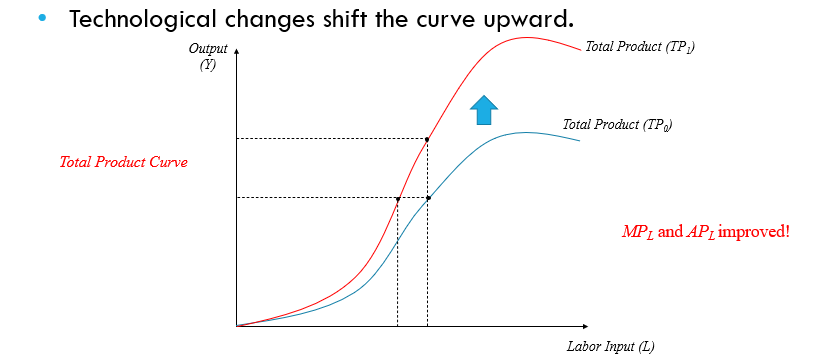
\includegraphics[width=0.7\linewidth]{technologicalChange}
\item \textbf{Economics of Digital Goods:} High fixed costs to produce the first unit, dominated by sunk cost: very high. Marginal production (reproduction) cost : very low. Hence, extensive economies of scale. Can be delivered via the Internet; little distribution cost.
\item DD and SS curve shifts as an impact of technological advances: Demand may shift leftward or rightward depending on the presence of substitutes or complements respectively. Supply increases generally as quality of product and cost of production changes due to technology.
\end{itemize}

\subsection{Disadvantages of Digital Economy}
\begin{itemize}
\item Digital divide: Generally refers to the gap between those who use or have access to telecommunications and information technologies including hardware, internet access, and literacy in using both effectively and those who do not.
\item Cybercrime and Privacy Breaches, Bad ideas spread quickly (e.g., fake news, racism, etc.), Pervasive Advertisement exposure (due to New business model), More monopolistic players (e.g., Google), Addictive nature of technology (Mental health and well-being concerns)
\end{itemize}

\textbf{Summary (of digital technology on businesses)}
\begin{itemize}
\item Digital technology enables economic activities such as production, distribution, and consumption of goods and services are conducted in a more efficient manner.
\item On top of that, digital innovation may lead to a fundamental change through a new economic rule, enhanced collaboration, and innovative business models.
\item However, some other challenges may also arise because of digital technologies
\end{itemize}






\end{multicols*}
\end{document}
